%test
% This is "sig-alternate.tex" V2.1 April 2013
% This file should be compiled with V2.5 of "sig-alternate.cls" May 2012
%
% This example file demonstrates the use of the 'sig-alternate.cls'
% V2.5 LaTeX2e document class file. It is for those submitting
% articles to ACM Conference Proceedings WHO DO NOT WISH TO
% STRICTLY ADHERE TO THE SIGS (PUBS-BOARD-ENDORSED) STYLE.
% The 'sig-alternate.cls' file will produce a similar-looking,
% albeit, 'tighter' paper resulting in, invariably, fewer pages.
%
% ----------------------------------------------------------------------------------------------------------------
% This .tex file (and associated .cls V2.5) produces:
%       1) The Permission Statement
%       2) The Conference (location) Info information
%       3) The Copyright Line with ACM data
%       4) NO page numbers
%
% as against the acm_proc_article-sp.cls file which
% DOES NOT produce 1) thru' 3) above.
%
% Using 'sig-alternate.cls' you have control, however, from within
% the source .tex file, over both the CopyrightYear
% (defaulted to 200X) and the ACM Copyright Data
% (defaulted to X-XXXXX-XX-X/XX/XX).
% e.g.
% \CopyrightYear{2007} will cause 2007 to appear in the copyright line.
% \crdata{0-12345-67-8/90/12} will cause 0-12345-67-8/90/12 to appear in the copyright line.
%
% ---------------------------------------------------------------------------------------------------------------
% This .tex source is an example which *does* use
% the .bib file (from which the .bbl file % is produced).
% REMEMBER HOWEVER: After having produced the .bbl file,
% and prior to final submission, you *NEED* to 'insert'
% your .bbl file into your source .tex file so as to provide
% ONE 'self-contained' source file.
%
% ================= IF YOU HAVE QUESTIONS =======================
% Questions regarding the SIGS styles, SIGS policies and
% procedures, Conferences etc. should be sent to
% Adrienne Griscti (griscti@acm.org)
%
% Technical questions _only_ to
% Gerald Murray (murray@hq.acm.org)
% ===============================================================
%
% For tracking purposes - this is V2.0 - May 2012

\documentclass[preprint]{sigplanconf-eurosys}

%\usepackage{amsmath}
\usepackage{courier}
\usepackage{listings}
\usepackage{amssymb}
%\usepackage{amsthm}
\usepackage{xcolor}
\usepackage{subcaption}
\usepackage{tabularx}
\usepackage{diagbox}
\usepackage{hyperref}
\usepackage[english,ruled]{algorithm2e}
\usepackage{multirow}
\usepackage{float}
\usepackage[pdftex]{graphicx}
\usepackage{color}
\usepackage{multirow}% http://ctan.org/pkg/multirow
\usepackage{hhline}% http://ctan.org/pkg/hhline


\newcommand*{\ttfamilywithbold}{\fontfamily{lmtt}\selectfont}

\definecolor{mygreen}{rgb}{0,0.6,0}
\definecolor{mygray}{rgb}{0.5,0.5,0.5}
\definecolor{mymauve}{rgb}{0.58,0,0.82}
\lstset{ %
  %emph={baz},
  %emphstyle=\textbf
  basicstyle=\scriptsize\ttfamily,        % the size of the fonts that are used for the code
  captionpos=b,                    % sets the caption-position to bottom
  commentstyle=\color{mygreen},    % comment style
  escapeinside={\%*}{*)},          % if you want to add LaTeX within your code
  showspaces=false,
  showstringspaces=false,
  framerule=1pt,
  frame=bt,	                   % adds a frame around the code
  keepspaces=true,                 % keeps spaces in text, useful for keeping indentation of code (possibly needs columns=flexible)
  keywordstyle=\bfseries,,       % keyword style
  language=Java,                 % the language of the code
  rulecolor=\color{black},         % if not set, the frame-color may be changed on line-breaks within not-black text (e.g. comments (green here))
  stringstyle=\color{mymauve},     % string literal style
  tabsize=2,	                   % sets default tabsize to 2 spaces
  title=\lstname                   % show the filename of files included with \lstinputlisting; also try caption instead of title
}



\begin{document}

\newcommand\VRule[1][\arrayrulewidth]{\vrule width #1}
\newcommand{\specula}{STR\xspace}

\title{STR: speculative execution for geo-replicated datastores}

\authorinfo{paper number XXX of XXX}
%\authorinfo{Zhongmiao Li$^{\dagger}$$^{\star}$, Peter Van Roy$^{\dagger}$ and Paolo Romano$^{\star}$ \\
%	 {\normalsize $^ {\dagger}$Universit\'e catholique de Louvain \quad
%          $^{\star}$Instituto Superior T\'ecnico} \\ [2mm]
%          \email{\{zhongmiao.li, peter.vanroy\}@uclouvain.be}\\
%          \email{\{zhongmiao.li, paolo.romano\}@ist.utl.pt}
%}


% There's nothing stopping you putting the seventh, eighth, etc.
% author on the opening page (as the 'third row') but we ask,
% for aesthetic reasons that you place these 'additional authors'
% in the \additional authors block, viz.

% Just remember to make sure that the TOTAL number of authors
% is the number that will appear on the first page PLUS the
% number that will appear in the \additionalauthors section.

\maketitle
\begin{abstract}

%The performance of geographically distributed data stores is challenged by the existence of ineluctably large communication delays between datacenters, which exacerbates the costs induced to ensure consistency of replicated data.
 This article introduces \specula (Speculative Transactional Replication), a geo-replicated transactional data-store that exploits speculative concurrency control techniques to mask the latency of inter data-center synchronization. \specula provides programmers with the flexibility to adopt, on a per transaction basis, either strong or weak consistency semantics.

On the one hand, the data replication protocol employed by \specula to ensure strong consistency, i.e., Snapshot Isolation (SI), departs from conventional designs, which  conservatively block transactions whenever they attempt to access data  updated by concurrently executing transactions. Conversely, \specula adopts a speculative approach, which avoids blocking transactions by allowing them to observe the data-item versions produced by concurrent (pre-committed) transactions. The evaluation indicates when there is non-trivial degree of local contention, the advantages stemming from embracing the risk of cascading aborts largely outweigh its drawbacks. On the other hand, \specula's weak consistency model, SPeculative Snapshot Isolation (SPSI), allow programmers to externalize the results of a transaction while this is still undergoing its commit/certification phase, hence allowing for further enhancing  throughput and latency. A key distinguishing treat of SPSI is that it provides clear and stringent guarantees on the atomicity and isolation of the snapshots observed and produced during transaction execution. This spares programmers from having to cope with complex concurrency bugs that could arise when using alternative weakly consistent models, like eventual consistency.

We performed an extensive evaluation, using a micro benchmark and two realistic workloads (TPC-C and RUBiS). The results show that comparing with a state-of-the-art transactional protocol, our strong consistency approach greatly increases throughput when there is non-trivial degree of local contention (which is the case for TPC-C and RUBiS), and allowing externalizing speculative results and pipelining transactions (the weak consistency model) reduces latency and even gives further speedup.
%This design choice allows \specula to achieve  up to XX$\times$ higher throughput and up to YY$\times$ lower latency than in state of the art strongly-consistent data stores., which suggests that, in geo-replicated datastores, the advantages stemming from embracing the risk of cascading aborts largely outweigh its drawbacks.
\end{abstract}




%
% The code below should be generated by the tool at
% http://dl.acm.org/ccs.cfm
% Please copy and paste the code instead of the example below. 
%

% We no longer use \terms command
%\terms{Theory}

\keywords{Speculative execution; geo-replication; transactional datastore}

\section{Introduction}
\label{sec:introduction}


Modern online services are increasingly deployed in multiple geographically-scattered datacenters (geo-replication)~\cite{spanner, kraska2013mdcc, li2012making}. Geo-replication allows services to remain available even in the presence of outages affecting entire data centers   and it reduces access latency by bringing data closer to clients. On the down side, though, the performance of geographically distributed data stores is challenged by the existence of unavoidably large communication delays between datacenters: two datacenters on opposite sides of the earth incur a minimal latency of 133ms, which is utterly bounded by the speed of light and can not be further reduced~\cite{bailis2013highly}. 

The inherently large synchronization overheads that affect geo-replicated data stores has a deep impact on the performance of the protocols employed to enforce data consistency. The problem is particularly exacerbated in  data-stores that i) support partial replication, and ii) ensure strong consistency semantics via ACID transactions --- two features that are recognized as highly desirable to enhance system's scalability~\cite{xxx} and simplify  applications' development~\cite{xxx}, respectively. 

For this class of systems, in fact, some form of global synchronization, typically based on a Two-Phase commit scheme~\cite{xxx}, is unavoidable in order to safely detect conflicts developed among  concurrent transactions executing at different data-centers. The adverse impact on performance of inter-data center synchronization is of a twofold nature: i) system's throughput can be severely impaired, as  transactions need to hold pre-commit locks during their global validation phase, which can cripple the effective concurrency that these systems can achieve; ii) client-perceived latency is also directly affected, since the inter-data-center  synchronization phase lies in the critical path of execution of transactions.


%This has motivated the investigation of a broad spectrum of data replication protocols for geo-replicated systems~\cite{xxx} as well as the exploration of diverse trade-off regarding the  consistency semantics offered to application developers~\cite{xxx}.

This work investigates the opportunities and challenges associated with the use of \textit{speculative} processing techniques in geo-distributed partially replicated transactional data stores  that provide a widely employed consistency criterion, i.e., Snapshot Isolation~\cite{xxx}. Generally speaking, speculative transactional processing techniques avoid to block transaction processing in presence of potential conflicts with concurrent transactions that would otherwise impose to wait for the completion of an inter-replica synchronization phase. Conversely, an optimistic assumption is made on how  such conflicts will be eventually resolved: if the assumption turns out to be correct, performance will benefit; else, in presence of a \textit{mispeculation}, the transaction has to undergo an abort.

We distinguish between two classes of speculative transaction processing techniques, which we call \textit{internal} and \textit{external} speculation,  depending on whether the effects of mispeculation are transparent or not for the programmers. Optimistic concurrency control~\cite{xxx} represents an instance of internal speculation. Conversely, asynchronous replication schemes~\cite{eventuallyconsistenttransactions} can be seen as an example of external speculation, as it requires programmers to develop compensation logic to cope with scenarios in which transactions have to be aborted \textit{after} their results have been already externalized.

In this paper we study how  to enhance performance of geo-distributed transactional data stores via two speculative techniques: \textit{speculative reads} and \textit{speculative commits}.

Speculative reads  allow a transaction T to immediately observe the  data item versions produced by a pre-committed transaction T', instead of blocking T until the outcome (abort/commit) of T' has been determined. Speculative reads are based on the optimistic assumption that pre-committed transactions will eventually be committed and belong to the class of internal speculation techniques, since  mispeculations can be managed fully transparently to the programmer by simply restarting T in case T' is aborted.


Speculative commits are instead an external speculative technique that allows for optimistically exposing the results produced by a transaction that this is still undergoing its global synchronization phase, under the assumption that no conflicts with remote transactions will be detected.

As we will also show via an extensive experimental study, both speculative reads and speculative commits can grant significant performance advantages in geo-distributed transactional data stores in case the optimistic assumptions on which they rely are met. Speculative commits can remove the global synchronization phase from the critical path of transaction execution, which normally a dominant role in the user perceived latency; 
 speculative reads can significantly reduce the ''effective´´ duration of pre-commit locks (i.e., as perceived by conflicting transactions), which not only reduces the transaction execution time but also enhances the maximum degree of parallelism achievable by the system --- and, hence, throughput.

However, the employment of these speculative techniques also raises two non-trivial challenges:
\begin{itemize}
\item Unless properly designed and intergrated in the underlying distributed concurrency control scheme, speculative transaction processing techniques may expose transactions to concurrency anomalies that would not otherwise arise and that would represent a source of additional complexity for application developers.
\item Speculation can hamper performance in adverse scenarios, where mispeculation occur excessively frequently. Also, the mechanisms employed to support speculation need to be extremely lightweight in order to minimize their overheads that may, otherwise, shadow or outweigh the theoretical performance gains that they may achieve.
\end{itemize}

{\bf reviewed up to here}

Data stores that embrace strongly consistent semantics, like Scatter~\cite{scatter} and Google's Spanner~\cite{spanner} are reckoned~\cite{shute2012f1} to greatly reduce the complexity of building distributed applications by providing programmers with the powerful abstraction of ACID transactions. However, it is also well known~\cite{brewer2012cap}  that enforcing strong-consistency requires introducing the latency of several inter-datacenter network round trips along the critical path of transactions' execution. This has not only a direct impact on the user-perceived latency --- a key discrimination factor for online services and a potential cause of large revenue losses  \cite{schurman2009user}, but also on throughput. In fact, throughout the execution of the replica synchronization protocol --- typically based on a Two-phase commit scheme~\cite{spanner,peluso2012score} --- existing strongly consistent data stores maintain, so called, pre-commit locks on the data items accessed by transactions. The duration of these locks, in geo-distributed data stores, can easily last on the order of a few hundreds of milliseconds. As a consequence, in workloads that generate non-minimal data contention, the probability of incurring lock convoying effects is greatly amplified, which can severely hinder the maximum throughput the system can withstand.

In order to tackle this problem, several systems have resorted to use weak consistency models, such as eventual consistency~\cite{kawell1988replicated, lloyd2011don, cure}, which allow to propagate transactions (or even individual operations, in case transactions are not supported) asynchronously. This brings remarkable benefits in terms of user-perceived latency and achievable throughput. These benefits, though, come at the cost of a significant increase of complexity for the application developers, who have to take responsibility of enforcing application's correctness in spite of a broad range of subtle concurrency anomalies~\cite{shute2012f1}. This includes developing compensation logic for transactions whose output has been externalized, in a speculative fashion, without waiting for the completion of the global certification phase: e.g., in an e-commerce application, handling the scenario in which a purchase order has to be eventually rejected or emended because the last stock of some requested item has been attributed to a concurrent transaction. Moreover, weak consistency models also require programmers to ensure that the application's logic does not break when transactions observe non-atomic snapshots that reflect only partially the effects of concurrent transactions or non-isolated snapshots that reflect the effects of conflicting transactions. This type of anomalies can be quite hard to predict or reason about, as they manifest as subtle concurrency bugs that can lead to anomalous system states, e.g., divisions by zero or infinite cycles~\cite{guerraoui2007opacity}, that may compromise the safety of user level applications, e.g., crashing them, and from which it is typically impossible to recover using business-level compensation logic.
\iffalse
In order to tackle this problem, in the literature various trade-offs have been explored between programming complexity and system performance by weakening the consistency semantics provided to programmers. some systems totally remove cross-site synchronous operations~\cite{kawell1988replicated, lloyd2011don, cure}; some reveals preliminary results to users to reduce latency, before operations finish execution~\cite{planet, icg}, and some systems that mix multiple consistency levels to reduce the latency of commutative operations~\cite{redblue, PSI}. Weakening system consistency brings remarkable benefits in terms of user-perceived latency and achievable throughput. These benefits, though, come at the cost of a significant increase of complexity for the application developers, including dealing with subtle concurrent anomalies, analyzing applications and writing compensation logics to emend the side-effect of externalized speculative results. 
\fi

%caused by observing data snapshots not producible by any sequential execution of transactions
\begin{figure}
\centering
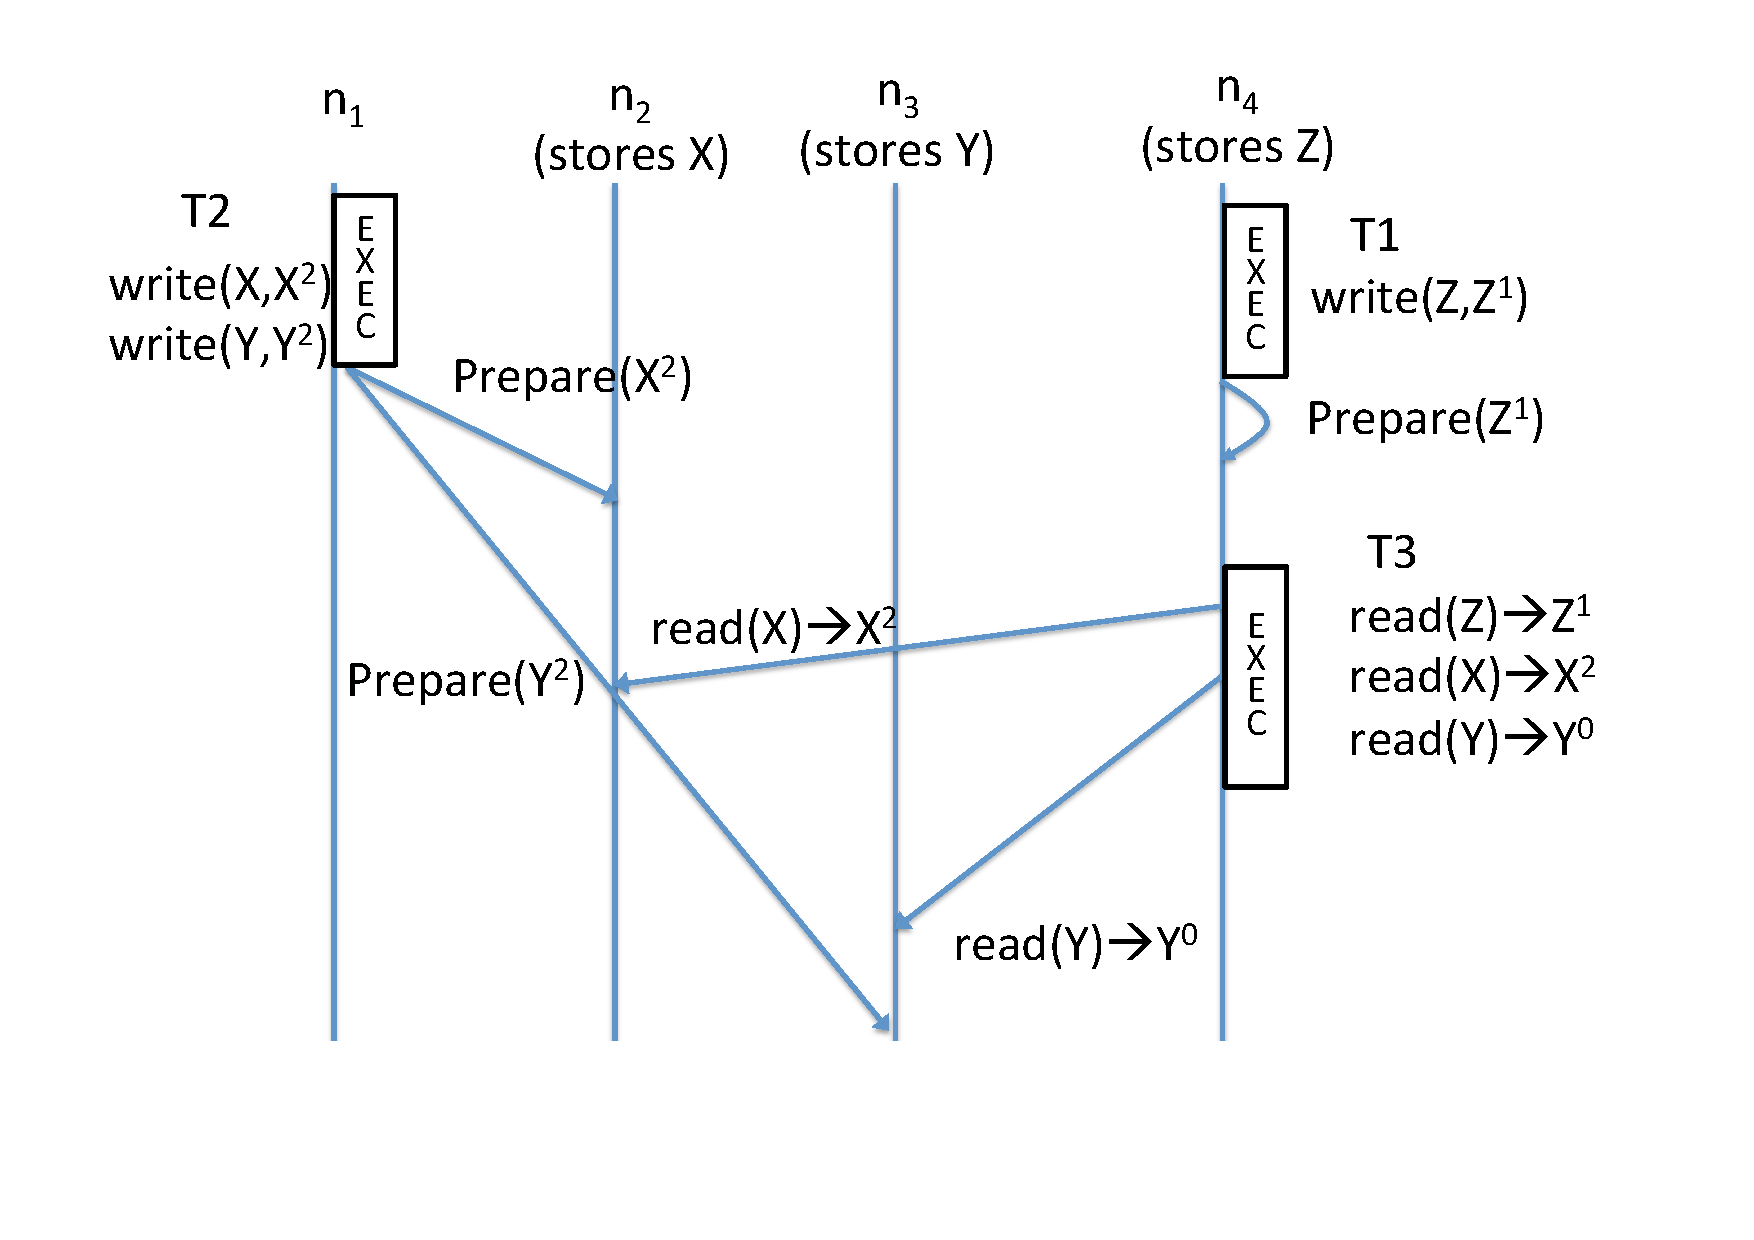
\includegraphics[scale = 0.24]{figures/example.pdf}
\caption{\footnotesize Example concurrency anomaly that may arise when adopting weak-consistency models that do not abide by the SPSI criterion.}
\label{fig:example}
\end{figure}

The system proposed in this paper, which we called \specula (Speculative Transactional Replication), provides developers with the flexibility of choosing between two different consistency semantics for the transactions that compose their applications: a strong consistency semantics, i.e., the familiar Snapshot Isolation~\cite{berenson1995critique}, and a weakly consistent one, which we termed Speculative Snapshot Isolation (SPSI). The idea of unifying different consistency models within the same programming model is not new: two notable examples are the red-blue consistency model recently proposed in Gemini~\cite{li2012making} and the support in SQL for specifying different isolation levels on a per transaction basis~\cite{sqk}.  The main innovative aspect of \specula lies in its novel transactional replication protocol, which provides unique advantages with respect to state of the art systems that provide either strong or weak consistency semantics (or both).

~\\
\noindent {\bf Strong consistency semantics:} 
\iffalse
The protocol employed by \specula to ensure strong consistency shares several key design choices with state-of-the-art data stores~\cite{spanner,clock-si,PelusoScore}, which contribute to its efficiency and scalability. These include:  multi-versioning, which maximizes efficiency in read-dominated workloads~\cite{bernstein-book},  distributed clocks, which are used to establish the transaction serialization order in a fully decentralized fashion,~\cite{spanner} as well as support for partial replication, a  feature that is generally regarded as fundamental to achieve high scalability~\cite{kemmeAndRicardo,PelusoGMU}. 
\fi
\specula supports transactions with strong consistency semantics, i.e. Snapshot Isolation, which provides programmers the familiar ACID properties. However, comparing with conventional transactional protocols, \specula takes a radically different approach regarding the management of transactional conflicts involving pre-committed data. Existing strong-consistent protocols take a conservative approach, which prevents any transaction T from ever observing the data item versions pre-committed by a different transaction T' --- either by blocking T till T' commits, or by letting T observe the pre-image of the execution of T'. This choice is arguably motivated by the fact that allowing transactions to observe pre-committed data item versions exposes them to the risk of cascading aborts~\cite{xxx}, a property that is ``historically'' deemed as crucial to maximize the efficiency of a transactional system~\cite{textbooks-on-db}. \specula departs from these conventional designs, and embraces a speculative approach that spares transactions that incur a conflict on pre-committed data from having to wait for the finalization of the commit phase of the lock-holding transaction. Conversely, \specula's distributed concurrency control mechanism takes an optimistic approach, i.e., it speculates on the eventual success (i.e., commit) of pre-committed transactions and allows the data versions pre-committed by a transaction T to be read by concurrent transactions, that are hence speculatively serialized after T. As we will show via an extensive experimental study, \specula's design choice of allowing speculative read can lead to increase throughput by up to XX$\times$ and reduce latency by up to YY$\times$. A striking, and more general, result stemming from our work is that, in strongly consistent geo-replicated data stores, the advantages stemming from accepting the risk of cascading aborts largely outweighs its drawbacks, leading to remarkable gains in terms of both throughput and latency.

~\\
\noindent {\bf Weak consistency semantics:} Analogously to the well-known eventual consistency model~\cite{brewer2012cap}, the weak consistency model supported by \specula, i.e., SPSI, allows application developers to \textit{speculative commit} transactions, i.e., to externalize to its users (e.g., human operators) the results of a transaction while this is still undergoing its final commit/certification phase. As such, when programmers choose to exploit the speculative commit capabilities of \specula, they also need to develop compensation logic for coping with the case in which a speculatively committed transaction has to be eventually aborted.

What distinguishes SPSI from existing weak consistency models is that it provides clear and stringent guarantees on the atomicity and isolation of the snapshots observed and produced during transactions' execution. Figure~\ref{fig:example} illustrates one of possible concurrency anomalies that can arise in a transactional system that adopts weak consistency, by exposing the data item versions produced by speculatively committed transactions: transaction T3 observes the version of data item X precommitted by a concurrent transaction, T2, on node n$_1$. However, when it comes to reading Y, which was also updated by T2, T3 misses the version created by T2 on node n$_3$ (as T2's updates are still being propagated to node \textit{n$_2$}). Such concurrency anomalies are prevented by the SPSI specification, which, in a nutshell, guarantees that the snapshots that can be observed/speculatively committed by a transaction T originated at a node \textit{n}
%
% observable by \textit{any} transaction (independently of whether they ) and those that are produced by a speculatively committed transaction T 
% 
 are equivalent to the ones that would have been observed/committed by T, had it been executed by a non-speculative SI data store along with a subset of all the transactions existing in the system, which excludes any concurrent, speculatively committed transaction originated at a node $n'\neq n$.
% 
% 
%  
% 
%  processed a subset of the entire set of transactions existing in the system that does include specu which comprises all the transactions that, by the time T started,  i) had either finalized their commit phase or ii) were activated on the same node that originated T and had speculatively committed.
 On the one hand,  SPSI  spares programmers from complex concurrency bugs, by ensuring that  transactions always execute on snapshots that are atomic and isolated, although not capturing the effects of concurrent, speculatively committed remote transactions. On the other hand, by demanding that the snapshots over which transactions execute reflect \textit{only} the effects of locally activated concurrent transactions, SPSI's specification allows for efficient implementations that can decide whether it is safe to speculatively commit a transaction solely on the basis of local information.

%, as illustrated in the example execution in Figure~\ref{example}, and ii) it makes transactions subject to cascading-aborts~\cite{xxx}, a property that is ``historically'' deemed as important for the efficiency of a transactional system. \specula rules out the former risk, thanks to an innovative, fully distributed, multi-versioned concurrency control scheme
%
%such data item to be ever observed, by blocking the  transaction requesting access to the data item or
%
%, though, departs from one of the key a
%
%
%
%Still, the latency and performance cost for guaranteeing consistency results seems indispensable. For example, logically a banking system should always be execute with strong consistency, as monetary loss caused by inconsistent operations seems unacceptable \cite{li2012making}. Interestingly, this is not always the case for systems used in daily life. Brew et al. described the design of a practical automated teller machine (ATM): when an ATM experiences network partition, it indeed takes the risk of overdrafting accounts to allows withdrawal unilaterally. In fact, ATM's ability to dispense money outweighs the trouble caused by account overdraft. Accidental overdraft will be handled by a well-defined external compensation logic \cite{brewer2012cap}.
%
%The design of the described ATM comes from a profound insight: practical applications may not always need 100\% consistency guarantee; instead, as long as the latency and availability benefit pay off the cost of compensating occasional mistakes, they may take risks, i.e. speculate on the result of operations, instead of pessimistically waiting out uncertainty \cite{helland2009building, brewer2012cap, bailis2013eventual}. In light of this, this paper presents {\specula}, a distributed transactional key-value store that exploits speculation to circumvent the inherent large latency and low throughput of strongly-consistent transactions. The main goal of \specula is to endow application developers the flexibility to speculate transactions for latency and throughput, while keeping programming complexity in check.
%
%\specula consists of a programming interface and a speculative transaction protocols. The programming interface allows programmers to exert control over speculative transaction: programmers develop application with strong consistency by default, but also have the choice to specify transactions to execute in a speculative fashion, without affecting other transactions. \specula 's speculative transactional protocol enables efficient transaction processing and ensures meaningful semantics, namely SPeculative Snapshot Isolation (SPSI), to programmers. Previous research works have exploited different aspects of speculation execution \cite{kraska2009consistency, pang2014planet}: Consistency Rationing \cite{kraska2009consistency} proposes cost models to measure the best tradeoff of consistency and cost; PLANET \cite{kraska2009consistency} proposes a speculative programming interface and calculates the commit probability of transactions. However, to the best of knowledge, we are the first to propose a speculative transactional protocol for modern large-scale, fully decentralized datastore.
% &  111 &  Haha &  Stupdi &  Noway & ahaha &   \\ \hline

Overall, this paper makes three main contributions:
~\\
\noindent {\em 1.} We propose SPeculative Snapshot Isolation (SPSI), a consistency criterion ad hoc designed for speculative transactional systems. SPSI extends the notion of Snapshot Isolation in an intuitive way, in order to provide meaningful consistency guarantees to transactions observing speculatively committed data (\S \ref{sec:overview}, \ref{sec:protocol}).
~\\
\noindent {\em 2.} We present the design of \specula, a  geo-replicated data store that exploits a novel, fully-decentralized, highly scalable protocol that efficiently supports speculatively transaction execution in presence of partially-replicated data  (\S \ref{sec:protocol}).
~\\
\noindent {\em 3.} We conduct an extensive experimental evaluation (\S \ref{sec:evaluation}),  encompassing both complex/realistic benchmarks (TPC-C and Rubis) and synthetic micro-benchmarks that allow us to exercise a wide range of diverse workloads. The results of our study highlight that:
\begin{itemize}
\item \specula's innovative speculative concurrency control ensures strong consistency (SI) with  average  gains of XX\% in throughput and YY\% in latency with respect to state of the art systems, with peak gains that extend up XX$\times$ for throughput and YY$\times$ for latency. 
\item Applications that adopt \specula's weak consistency semantics (SPSI) can reduce the user-perceived latency, on average  (i.e., considering both scenarios of successful and unsuccessful speculation), by an additional XX\% factor. Further, \specula's weak consistency semantics   allow for enhancing the throughput achievable by \specula by up to XX$\times$ in machine-to-machine applications in which the rate of submission of new transactions is solely throttled by the speed at which the system can process previously submitted transactions.
\end{itemize}

The remainder of this paper is structured as follows. {\bf TODO}


\section{Background and Related Work}
\begin{table*}
\small
\begin{center}
  \begin{tabular}{ c | c | c | c | c | c } 
      \multirow{2}{*}{\textbf{Systems}} & \multicolumn{2}{c|}{\textbf{Performance benefits}} &  \multicolumn{3}{c}{\textbf{Programming complexity}}   \\ \hhline{~-----}
       & Throughput & Latency & Program analysis & Concurrency bugs & Compensation logic \\ \hline
       COPS~\cite{lloyd2011don}/GentleRain~\cite{du2014gentlerain} &  Yes & Yes & N/A & Yes & Yes \\ \hline
       Gemini~\cite{li2012making} & Blue ops & Blue ops & Yes & No & No \\ \hline
       Consistency Rationing~\cite{kraska2009consistency} & Weak ops & Weak ops & Yes & Yes & Weak ops \\ \hline
       Salt Isolation~\cite{xie2014salt} & Base ops & Base ops & No & Base ops & N/A \\ \hline
       PLANET~\cite{pang2014planet}/ICG~\cite{icg} &  No  & Spec ops  & No & No & Spec ops \\ \hline
       STR &  Yes*  & Spec ops & No & No & Spec ops \\ \hline
  \end{tabular}
\end{center}
\caption{Maximal mean latency of a DC to its replicas and to all other DC}
\label{tab:related}
\end{table*}

\paragraph{Tradeoffs between performance and programming complexity} In the literature, various tradeoffs have been explored between programming complexity and system performance, which have intrigued different design of distributed datastores. These consistency models range from eventual consistency (causal consistency), which totally avoids synchronization among data replicas, to systems that mix strong and weak consistency levels. We start by listing different aspects of performance benefits as well as programming burdens that these models may bring, compared with a strongly-consistent model.

Two desirable performance improvement that can be brought by weakening consistency guarantees are \textbf{latency} and \textbf{throughput}. Low access latency is crucial for the user experience of online services, while higher throughput means a system is able to handle more concurrent requests. On the other hand, a weak consistency model may bring extra complexity for application developers. A most notable complexity is to cope with \textbf{concurrency anomalies}. In contrast to the ACID properties provided by conventional transactions, applications of a weakly-consistent datastore can observe effects of non-isolation, i.e. intersecting conflicting, transactions or partial updates of a transaction that requires ad-hoc logics to handle. Furthermore, some systems~\cite{helland2009building, icg, pang2014planet} choose to expose preliminary results of some operations to mask large operation latency, which requires programmers to write \textbf{compensation logic} for these operations in case they are incorrect and need to be emended. Last but not least, some systems mix multiple consistency levels, which requires a thorough \textbf{program analysis}, essentially to analyze possible interactions between all operations to ensure that executed some operations under weaker consistency will not compromise the correctness of applications.

\paragraph{Representative systems} In table \ref{tab:related}, we compare STR with several representative distributed datastores that relax consistency semantics to trade for better performance. Causally-consistent systems, like COPS~\cite{lloyd2011don} and GentleRain~\cite{du2014gentlerain}, propagate transactions asynchronously to remote datacenters (DCs). As no inter-DC synchronous is needed, these systems provide low operation latency and high throughput. However, this weak model can not prevent occurrence of concurrent conflicting transactions from different DCs, which causes concurrency anomalies and may need to be compensated.

Gemini~\cite{li2012making} requires programmers to analyze applications and identify (possibly with the aid of static analysis tools~\cite{atc-rodrigo}) which subset of application's operations commute and can safely take advantage of weak consistency semantics (blue operations). On the other hand, unlike STR, Gemini does not improve the performance of red operations (strongly-consistent operations).

Xie et. al.~\cite{xie2014salt} propose Salt Isolation, which allows classic ACID transactions to co-exist with BASE transactions, i.e., weakly consistent transactions that can externalize their intermediate state to minimize lock duration. Analogously to SPSI, Salt ensures that strong consistent transactions are not affected by the execution of weak consistent ones. Though, weakly consistency transactions (BASE) may observe the intermediate states of each other, which raises concurrent anomalies. On the contrary,  \specula ensures that \textit{any} transaction, even the ones that execute with weak consistency semantics, always observe and produce atomic and isolated snapshots (although potentially not reflecting the execution of concurrent transactions originated at different nodes).

Kraska et. al. allows programmers to specify which data shards demand strong consistency (serializability) and which ones can tolerate weak semantics (session guarantees), albeit possibly at some cost. This information is then exploited to dynamically adapt the consistency provided to transactions and reach an optimal balance between consistency and latency \cite{kraska2009consistency}. Unlike \specula, though, this approach only guarantee the weakest consistency semantics to transactions that access both weakly and strongly consistent data shards, which can not spare programmers from the need of handling concurrency bugs. Weak operations are speculative, therefore compensation logic is needed in case later on they have to be undone. \textbf{Make sure if program analysis is needed}.

PLANET~\cite{pang2014planet} and Incremental Consistency Guarantees (ICG)~\cite{icg} have explored the idea of exposing preliminary results, instead of final results that are produced after a global execution, to users to reduce perceived latency. The programming model exposed by PLANET and ICG aim to reduce the user-perceived latency by letting programmers expose the results of speculatively committed transactions. Unlike \specula, though, PLANET relies on a conventional/non-speculative data replication scheme that  never exposes pre-committed data to transactions. As such, PLANET can only benefit user-perceived latency, but fails to reduce the transaction's blocking time and, hence, to enhance throughput and reduce the time it takes to finalize the processing of a transaction. ICG does not support transactions, and delivering preliminary results brings considerable overhead. 

\iffalse
Recently, several datastores have been proposed that ensure strong consistency semantics in geo-replicated settings. Two notable examples are Spanner \cite{spanner} and Scatter \cite{scatter}, which provide Serializable transactions via the use of Two-phase commit and Paxos. In order to reduce commit latency in geo-replicated settings, some protocols have proposed variants of these techniques based on the assumption that data is fully replicated across different data-centers, i.e., each data-center maintains a full image of the system's data. To this end, Replicated Commit~\cite{mahmoud2013low} runs Two-Phase Commit multiple times in different datacenters and then uses Paxos to reach consensus as to whether the transaction should commit; MDCC~\cite{kraska2013mdcc} uses Generalized Paxos \cite{lamport2005generalized} to commit transaction, which takes only a single WAN round-trip in normal case. Unlike these works, \specula supports a more generic and scalable data-model, in which data can be partially replicated across a subset of the available data-centers.

An alternative approach that has been intensively explored in literature, and which also \specula supports, consists in supporting the simultaneous execution of transactions that use strong and weak consistency models. Gemini~\cite{li2012making} requires programmers to analyze applications and identify (possibly with the aid of static analysis tools~\cite{atc-rodrigo}) which subset of application's operations commute and can safely take advantage of weak consistency semantics.  Unlike \specula, Gemini, assumes a fully replicated data model and, as such, it does not address the issue of how to achieve isolation in presence of operations/transactions that require accessing  multiple data items scattered across different machines (see Figure~\ref{fig:example}).

Other recent approaches~\cite{zhang2013transaction,SwiftCloud,Walter} have aimed to reduce the cost of enforcing strong consistency, e.g., by identifying (possibly in a semi-automatic way) and exploiting the presence of commutative operations that can be executed without endangering consistency (as they are guaranteed to never conflict). Bumper~\cite{Diegues2013SRDS}  focuses on the problem of contention hot-spots, allowing to postpone the execution of conflict-prone operations issued within a transaction till their commit phase --- where they are executed after having acquired all the locks they require, and hence without risking to incur aborts. These approaches are orthogonal to \specula and  these mechanisms  could be combined with the speculative techniques  at the heart of \specula's replication protocol to further enhance its performance.

As discussed in \S \ref{sec:introduction}, this design choice spares programmers from the complexity of reasoning on subtle concurrency bugs that may lead applications running in non-sand-boxed environments  to exhibit arbitrary behaviours~\cite{opacity, virtualWorldConsistency}: this is the case, for instance, of applications that do not access data via well-defined query languages, like SQL, but rather by embedding transactions into arbitrary code written in a general purpose programming language, like Java~\cite{javaPersistenceAPI}. While, in the former case, inconsistencies lead to stale data being returned, but will not cause the data-store to crash, in the latter case, inconsistencies can lead applications to crash because of unexpected exceptions or to enter infinite loops~\cite{transactionsAreBackButTheyAreNotTheSame}. 

Unlike \specula, Gemini, assumes a fully replicated data model and, as such, it does not address the issue of how to achieve isolation in presence of operations/transactions that require accessing multiple data items scattered across different machines (see Figure~\ref{fig:example}).
\fi
 
\textbf{Other related work} Recently, several datastores have been proposed that ensure strong consistency semantics in geo-replicated settings. Two notable examples are Spanner \cite{spanner} and Scatter \cite{scatter}, which provide Serializable transactions via the use of Two-phase commit and Paxos. In order to reduce commit latency in geo-replicated settings, some protocols have proposed variants of these techniques based on the assumption that data is fully replicated across different data-centers, i.e., each data-center maintains a full image of the system's data. To this end, Replicated Commit~\cite{mahmoud2013low} runs Two-Phase Commit multiple times in different datacenters and then uses Paxos to reach consensus as to whether the transaction should commit; MDCC~\cite{kraska2013mdcc} uses Generalized Paxos \cite{lamport2005generalized} to commit transaction, which takes only a single WAN round-trip in normal case. Unlike these works, \specula supports a more generic and scalable data-model, in which data can be partially replicated across a subset of the available data-centers.

The idea of letting transactions ``optimistically'' borrow, in a controlled manner, the updated data of transactions currently in their commit phase has already been investigated in the past. Several works, e.g., SPECULA \cite{peluso2012specula} and Aggro \cite{palmieri2010aggro}, have applied this idea in contexts that are radically different from the ones considered in this paper, i.e., small scale clusters in which data is fully replicated via total-order based coordination primitives whereas \specula is designed for partially replicated data-stores distributed over geographical scale that ensure consistency via Two-phase commit.  SCC-kS~\cite{bestavros1996value}, PROMPT~\cite{PROMPT} and SL~\cite{Reddy} target a relatively closer system model, i.e., distributed databases, but do not support data replication and multi-version concurrency control, two mechanisms that are regarded as essential in modern, large scale online services~\cite{spanner,megastore,score}. Further, some of these proposals ~\cite{bestavros1996value, Romano-2014} rely on complex graph-based concurrency control techniques, whose efficiency has also been evaluated via simulation and that are likely to suffer from large overheads in realistic settings. Finally, unlike \specula PROMPT, SL and SCC-kS may expose non-atomic/isolated snapshots during transaction's execution.











\section{Conclusion}
This paper proposed {\specula}, a novel protocol that uses speculative techniques to improve performance of distributed transactions. The three novel speculative techniques, i.e. speculative commit, speculative read and precise clock, collectively mitigate the performance bottleneck of existing transactional protocol. Extensive benchmark showed that our protocol achieves significantly higher throughput than state of the art non-speculative system and is particularly beneficial when workloads have high local conflict and low remote conflict.


% We recommend abbrvnat bibliography style.
\bibliographystyle{abbrv}
\bibliography{references}
\end{document}
